\chapter{Der Brentanoraum}\label{chap:bs}

In diesem Kapitel wird in Grundzügen die von Baumann, Herre und Loebe entwickelte Axiomatisierung des Brentanoraumes $\theoryBS$ dargestellt und auf dieser Grundlage die Theorie $\theoryBSO$ der ordinären Raumentitäten eingeführt.
Dabei fokussiere ich mich auf einige relevante Aspekte.
Eine vollständige Übersicht findet sich auf den entnehmbaren Übersichtsblättern (Übersicht~1 für $\theoryBS$ und Übersicht~2 für $\theoryBSO$) 


\section{Primitive Relationen}\label{sec:bsprimitive}
Die in [\cite{baumann-r-2016-53-a}] vorgestellte Axiomatisierung des Brentanoraumes baut auf vier primitiven Relationen auf, nämlich Raumregionen (space regions), räumliche Grenzen (spatial boundaries), Koinzidenz (coincidence) und räumlicher Teil (spatial part). 
%Tabelle \ref{tab:symbole} im Anhang liefert einen Überblick über die zugehörigen Symbole.


%\begin{enumerate}

 %\item \textbf{Raumregion (space region):} 
\paragraph{Raumregion:}
%\paragraph{}
       %\spacedlowsmallcaps{Raumregionen} 
       Raumregionen
       \marginpar{Raumregion,\\phänomenologischer Raum}
       sind Instanzen des sogenannten phänomenologischen Raumes (phenomenal space), welcher erzeugt wird durch materielle Objekte und deren räumliche Beziehungen untereinander.
       Ein materielles Objekt erzeugt eine Raumregion, indem es sie einnimmt. 
       Beispielsweise kann der Raum, den unsere Sonne einnimmt, als Raumregion betrachtet werden.
       Nicht nur materielle Objekte, sondern auch Aggregate materieller Objekte können Raumregionen erzeugen.
       Unser Sonnensystem zum Beispiel, also die Sonne und die sie umkreisenden Planeten, erzeugt
       %Beispielsweise erzeugt unser Sonnensystem, also unsere Sonne, die sie umkreisenden Planeten und deren natürliche Satelliten, die Zwergplaneten und andere Kleinkörper wie Kometen, Asteroiden und Meteoroiden sowie die Gesamtheit aller Gas- und Staubteilchen, die durch die Anziehungskraft der Sonne an diese gebunden sind, 
       eine nichtzusammenhängende Raumregion.
       Symbolisch besagt $\GSReg(x)$, dass $x$ eine Raumregion ist.
       Zur Vereinfachung wird im Folgenden nicht mehr zwischen (Aggregaten) materieller Körper und  den von ihnen erzeugten Raumregionen differenziert und beispielsweise das Sonnensystem als Raumregion betrachtet.
   
 %\item \textbf{Räumliche Grenze (spatial boundary):}
 \paragraph{Räumliche Grenze:}
 %\paragraph{}
        %\spacedlowsmallcaps{Räumliche Grenzen} 
        Räumliche
        \marginpar{Räumliche Grenze,\\niederdimensionale Raumentität}
        Grenzen sind Teilmengen der Ränder von Raumentitäten.
        Die binäre Relation $\Gsb(x,y)$ drückt aus, dass die Raumentität $x$ die Raumentität $y$ begrenzt. 
        Beispielsweise begrenzt die Erdoberfläche die Erde, aber auch der Teil der Erdoberfläche, der von der Antarktis eingenommen wird, gilt als Grenze unseres Planeten.
        Die Küstenlinie der Antarktis wiederum begrenzt diesen Kontinent.
        Im Gegensatz zur gesamten Küstenlinie, die keine Grenzen hat, werden deren Abschnitte durch ihre Endpunkte begrenzt.
        
        Eine Raumentität kann mehr als eine andere begrenzen. Die Küstenlinie von Japan beispielsweise begrenzt sowohl Japan als auch die Landflächen der Erde, nicht jedoch deren Wasserflächen (siehe Koinzidenz).
        
        In diesem Sinne erzeugt die $\Gsb$-Relation aus Raumregionen $2$-dimensionale Raumentitäten, diese wiederum $1$-dimensionale und diese $0$-dimensionale.
        $2$-, $1$- und $0$-dimensionale Raumentitäten werden als niederdimensional bezeichnet.
        
%  
%        Raumregionen bilden die 3-dimensionalen Raumentitäten (space entities).
%        Niederdimensionale Raumentitäten existieren als Grenzen von höherdimensionalen
%        \footnote{oder als mereologische Summe von solchen}
%        .
%        Die binäre Relation $\boldsymbol{\Gsb(x,y)}$ drückt aus, dass die Raumentität $x$ die Raumentität $y$ begrenzt. 
%        Eine Raumentität muss eine andere jedoch nicht komplett umschließen, um als deren Grenze zu gelten.
%        Beispielsweise begrenzt die Erdoberfläche die Erde, aber auch der Teil der Erdoberfläche, der von der Antarktis eingenommen wird, gilt als Grenze unseres Planeten.
%        Die Küstenlinie der Antarktis wiederum begrenzt diesen Kontinent.
%        Im Gegensatz zur gesamten Küstenlinie, die keine Grenzen hat, werden deren Abschnitte durch ihre Endpunkte begrenzt.
%        Eine niederdimensionale Raumentität kann mehr als eine höherdimensionale begrenzen. Die Küstenlinie von Japan beispielsweise begrenzt sowohl Japan als auch die Landflächen der Erde, nicht jedoch deren Wasserflächen (siehe Koinzidenz).

 %\item %\textbf{Koinzidenz (coincindence):} 
    \paragraph{Koinzidenz:}
    %\paragraph{}
       Ein
       \marginpar{Koinzidenz}
       charakteristisches Merkmal des Brentanoraumes ist, dass dort, wo zwei gleichdimensionale Raumentitäten aneinanderstoßen, jede ihre eigene Grenze hat (siehe Abbildung \ref{fig:kastanie}).
       Liegt beispielsweise ein Buch auf einem Tisch, so werden die untere Seite des Buches und der Teil der Tischfläche, auf dem das Buch liegt, als unterschiedliche Raumentitäten betrachtet. 
       Wir sagen, die beiden Flächen %\spacedlowsmallcaps{koinzidieren}
       koinzidieren. 
       D.\,h.\ sie berühren einander, sind aber nicht notwendigerweise gleich. 
       In diesem Sinne wäre die Küstenlinie von Japan, wenn sie als Grenze des Landes betrachtet wird, \emph{keine} Grenze der Wasserflächen der Erde.
       Das Prädikatensymbol $\Gscoinc(x,y)$ besagt, dass die Raumentitäten $x$ und $y$ koinzidieren.
       Koinzidenz ist eine Äquivalenzrelation auf den sogenannten ordinären, niederdimensionalen Raumentitäten (zum Begriff der Ordinärität s.\,u.). 
       Das bedeutet insbesondere, dass jede niederdimensionale Raumentität mit sich selbst koinzidiert.
           
        \begin{figure}[ht]
            \centering
            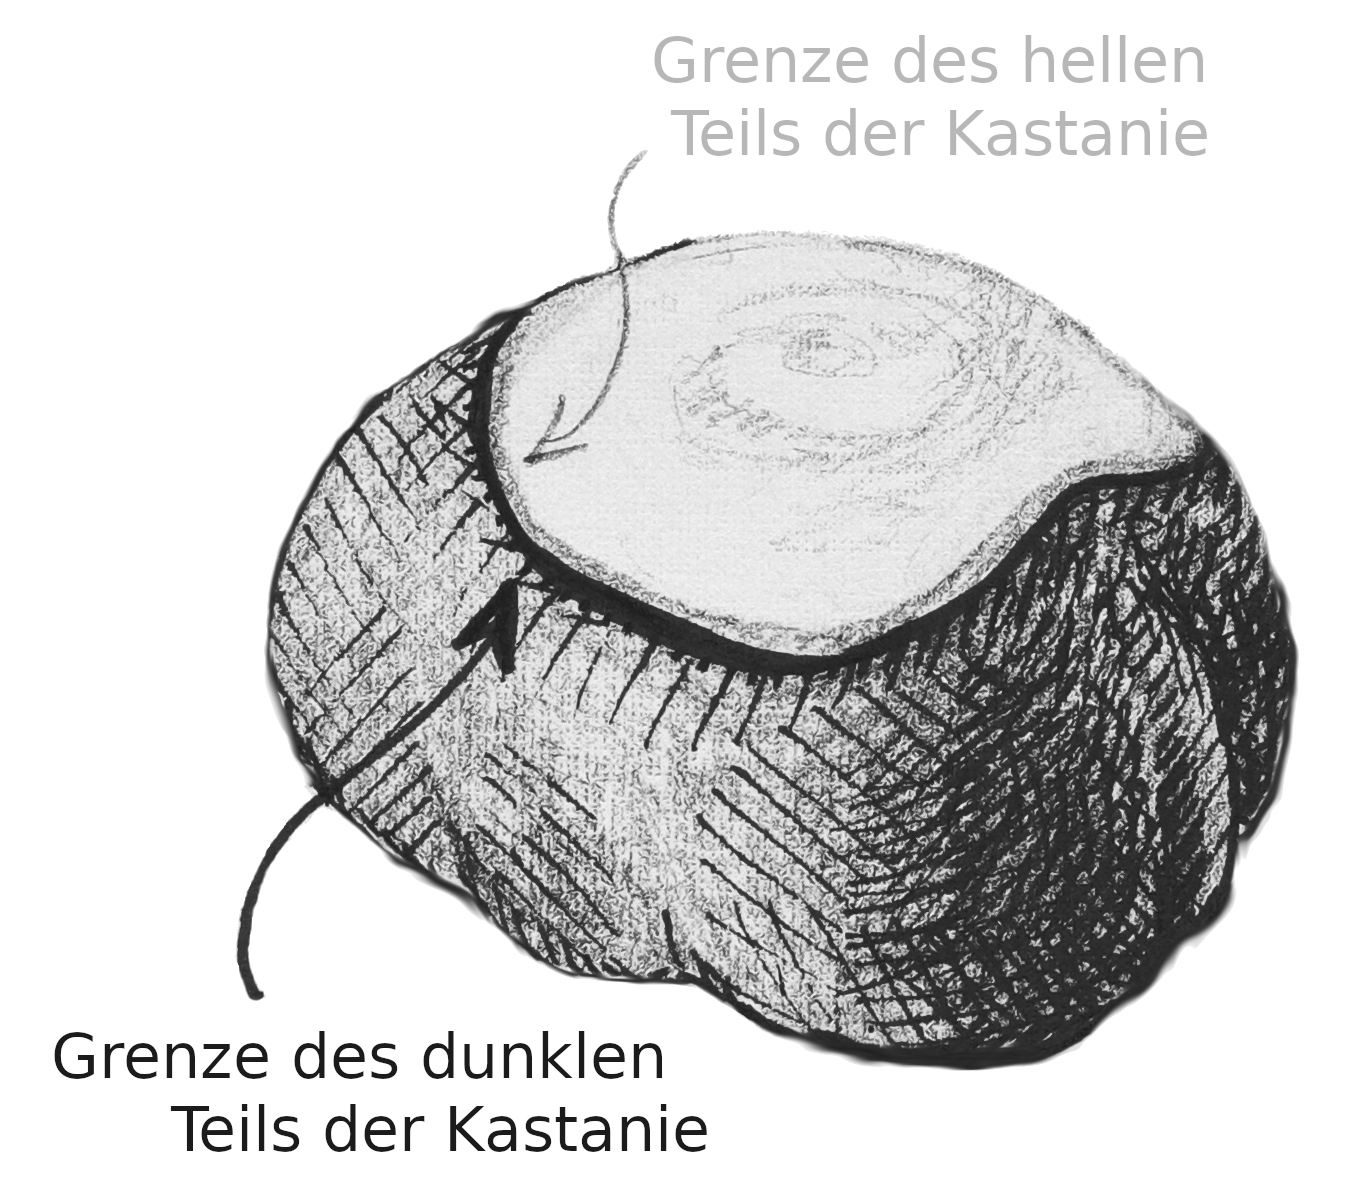
\includegraphics[height=4cm]{abb/kastanie.png}
            \caption{Jede Grenzfläche hat ihre eigenen Grenzlinien}
            \label{fig:kastanie}
        \end{figure}
        
       
 %\item \textbf{Räumlicher Teil (spatial part):}
 \paragraph{Räumlicher Teil:}
 %\paragraph{}
       Raumentitäten
       \marginpar{Räumlicher Teil}
       können Teil anderer gleichdimensionaler Raumentitäten sein.
       Sachsen ($2$-dimensional) ist beispielsweise ein Teil Deutschlands ($2$-dimensional), nicht jedoch die sächsische Grenze zwischen Sachsen und Thüringen ($1$-dimensional).
       Mit $\Gspart(x,y)$ wird ausgedrückt, dass $x$ ein räumlicher Teil von $y$ ist.
       Bei Raumregionen entspricht die $\Gspart$-Relation dem intuitiven Verständnis der Teil-von-Beziehung. 
       Der Erdkern ist beispielsweise ein Teil der Erde.
       Wenn eine niederdimensionale Raumentität $A$ eine andere begrenzt, so wird diese auch von jedem Teil von $A$ begrenzt.
       % Eine niederdimensionale Raumentität kann nur Teil einer anderen sein, wenn sie eine gleiche höherdimensionale Raumentität begrenzen.
       % Genauer gesagt: Wenn $A$ Grenze von $B$ ist und $A'$ Teil von $A$, so muss auch $A'$ Grenze von $B$ sein.
       
%\end{enumerate}


\section{Ausgewählte definierte Relationen}
In diesem Abschnitt stelle ich ausgewählte definierte Relationen der Theorie $\theoryBS$ anschaulich vor. 
%Eine vollständige Liste aller definierter Relationen sowie ihrer formalen Definitionen findet sich im Anhang \ref{anh:def-rel-bs}.
    
    \paragraph{Räumliche Grenzen und niederdimensionale Raumentitäten:}
    %\paragraph{}
        %SB, dDE, LDE, eqdim
        Eine
        \marginpar{Räumliche Grenze,\\niederdimensional,\\gleichdimensional,\\Flächen-/Linien-/Punktregion}
        räumliche Grenze (spatial boundary) ist eine Raumentität, die eine andere begrenzt%
        \footnote{Dies ist nicht zu verwechseln mit der binären $\Gsb$-Relation, bei der $\Gsb$ auch für \glqq spatial boundary\grqq\ steht.}.
        Niederdimensionale Raumentitäten sind Raumentitäten, die keine Raumregionen sind. 
        Sie haben immer einen Teil, der eine andere Raumentität begrenzt.
        Es gibt jedoch niederdimensionale Raumentitäten, die nicht als Ganzes Grenze einer anderen sind (vgl.\ extraordinäre Raumentitäten unten).
        Raumentitäten, die einen Teil haben, der eine $n$-dimensionale Raumentität begrenzt sind $(n-1)$-dimensional ($n \in \{1,2,3\}$).
        Die $\Geqdim$-Relation besagt, dass zwei Raumentitäten die gleiche Dimension haben.
        Niederdimensionale Raumentitäten werden je nach Dimension -- in üblicher Weise -- Flächen-, Linien- oder Punktregionen genannt.
        
    \paragraph{Teile und Hyperteile:}
        %sppart, inpart, hypp, sov
        Die
        \marginpar{echter Teil,\\atomare Raumentität,\\Überlappung,\\Hyperteil,\\innerer/tangentialer Teil}
        $\Gspart$-Relation ist eine partielle Ordnung. Die zugehörige strikte partielle Ordnung (echter räumlicher Teil) wird mit $\Gsppart$ (proper spatial part) bezeichnet.
        Eine Raumentität, die keinen echten Teil besitzt, heißt atomar.
        Zwei gleichdimensionale Raumentitäten überlappen (overlap), wenn sie einen Teil besitzen, der beiden gemeinsam ist (siehe Abbildung \ref{fig:overlap}).
        Die $\Gspart$-Relation stellt eine Beziehung zwischen gleichdimensionalen Raumentitäten dar.
        Die Hyperteil-Relation hingegen drückt aus, dass eine Raumentität in einer anderem mit höherer Dimension enthalten ist.
        Je nach Dimension der niedriger-dimensionalen Raumentität spricht man von $2$-, $1$- oder $0$-dimensionalen Hyperteilen.
        Hyperteile können sowohl ganz im Inneren einer anderen Raumentität liegen als auch auf deren Rand.
        Ein innerer Teil einer Raumentität ist ein räumlicher oder ein Hyperteil, der nicht ihren Rand berührt. 
        Ansonsten spricht man von einem tangentialen Teil.
        Da Punktregionen keinen Rand haben, bestehen sie nur aus inneren Teilen.
        Innere und tangentiale Teile müssen jedoch nicht unbedingt Hyperteile sein, sondern können auch gleichdimensional und in diesem Fall räumliche Teile sein.
        Abbildung~\ref{fig:hypp} zeigt verschiedene Fälle der Hyperteil-Beziehung sowie Beispiele für innere und tangentiale Teile.
        
        %\todo[inline]{Bild hypp einscannen}
        \begin{figure}[ht]
            \centering
            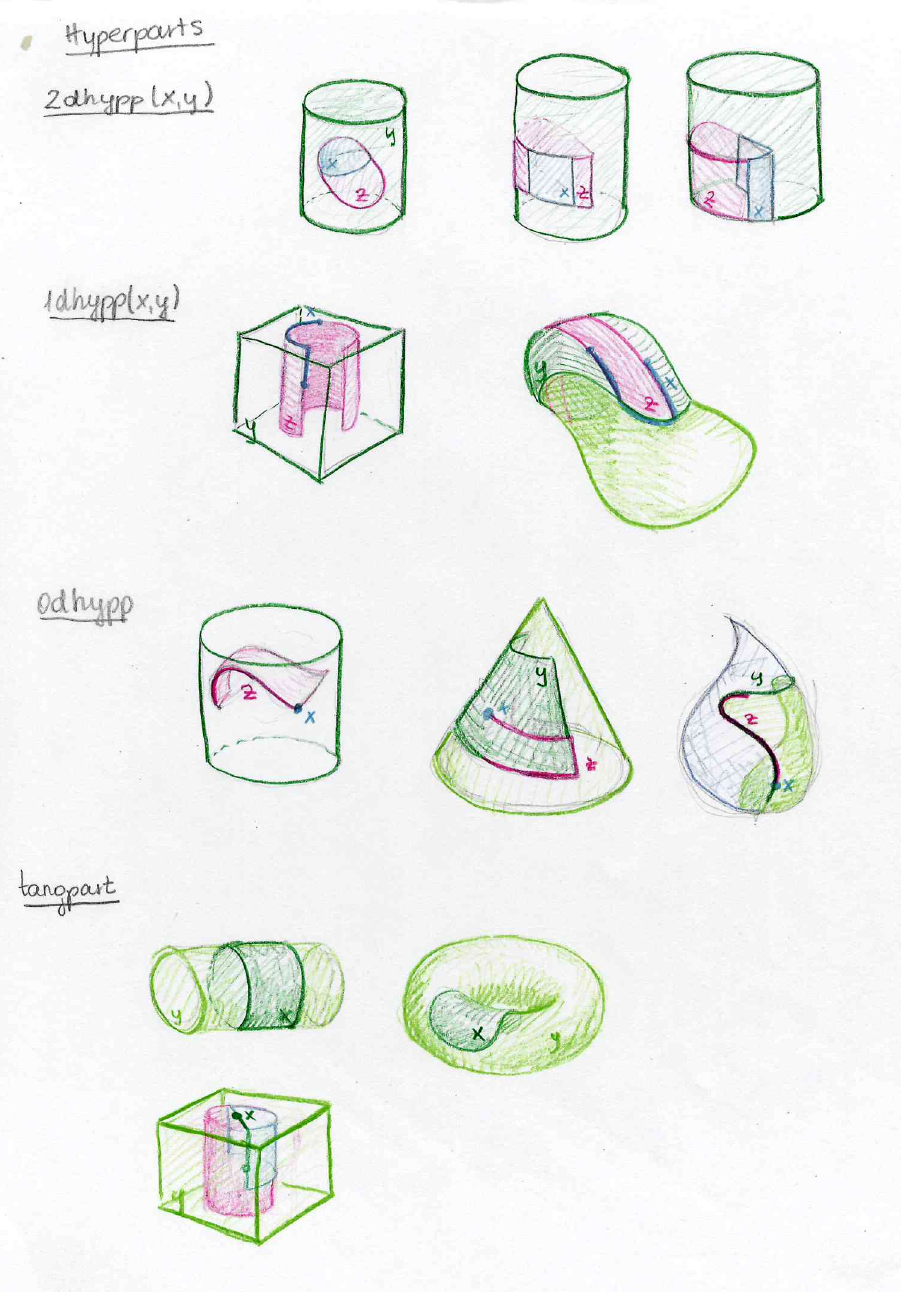
\includegraphics[width=10cm]{bearbeitet-22-04-25/hypp.png}
            \caption{Verschiedene Fälle von Hyperteilen}
            \label{fig:hypp}
        \end{figure}

    \paragraph{Mereologische Summe, ordinäre und extraordinäre Raumentitäten:}
        Die
        \marginpar{mereologische Summe,\\ordinär,\\extraordinär}
        mereologische Summe zweier Objekte ist eine Entität, die die gleichen Teile besitzt wie die beiden ursprünglichen.
        Beispielsweise ist die mereologische Summe von Europa und Russland die Landfläche, die Europa und Russland gemeinsam einnehmen (siehe Abbildung \ref{fig:mereologische-summe}).
        Als Spezialfall ist die mereologische Summe eines Objekts mit einem Teil von sich selbst wieder das Objekt selbst.
%         In $\BS$ können mereologische Summen nur aus Entitäten gleicher Dimension gebildet werden.
%         Wenn die beteiligten Entitäten Teile besitzen, die zwar koinzidieren, aber nicht gleich sind entstehen dabei extraordinäre Raumentitäten. 
%         Haben wir beispielsweise zwei aufeinanderliegende Würfel und betrachten die mereologische Summe ihrer Oberflächen, so koinzidert die Oberseite des unteren mit der Unterseite des oberen und es entsteht eine extraoordinäre Raumentität.
%         Zur Definition der mereologischen Summe in der Theorie $\BS$ wird die Überlappungsrelation $\Gsov(x,y)$ benutzt, die besagt, dass $x$ und $y$ einen gemeinsamen Teil haben.
%         Damit wird definiert: $\Gsum(x,y) := \fa u (\Gsov(x,u) \oder \Gsov(y,u) \leftrightarrow \Gsov(z,u))$.
        \begin{figure}[ht]
            \centering
            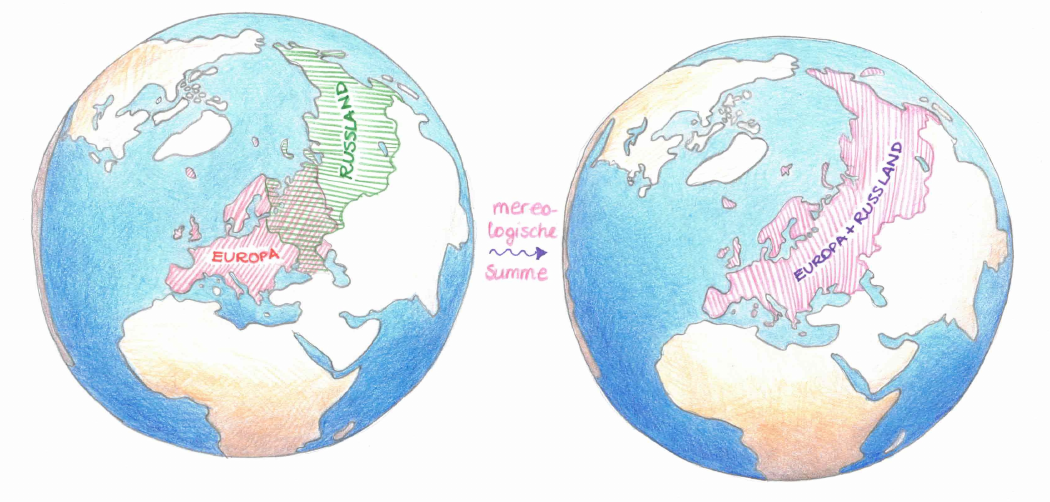
\includegraphics[width=\textwidth]{gfx/mereologische-summe.png}
            \caption{Mereologischen Summe von Flächenregionen}
            \label{fig:mereologische-summe}
        \end{figure}
        %
		Raumregionen und räumliche Grenzen sind ordinäre Raumentitäten.
		Die Theorie fordert die uneingeschränkte Existenz der mereologischen Summe gleichdimensionaler Entitäten. Dadurch können extraordinäre Raumentitäten entstehen. Das sind Raumentitäten, die Teile haben, die koinzidieren, aber nicht überlappen.
		Nehmen wir die Oberflächen zweier übereinanderliegenden Würfel. 
		Die obere Fläche des unteren Würfels koinzidiert mit der unteren Fläche des oberen Würfels. Die beiden Flächen haben jedoch keine Teile gemeinsam, da die erste von unten, die zweite von oben erzeugt wird. 
		Mit anderen Worten: Sie überlappen nicht. Damit ist ihre mereologische Summe eine extraordinäre Raumentität.
		Ein ähnliches Beispiel ist in Abbildung \ref{fig:extraordinaer} dargestellt.
		%
		%\todo[inline]{Bild extraordinaer einscannen}
        \begin{figure}[ht]
            \centering
            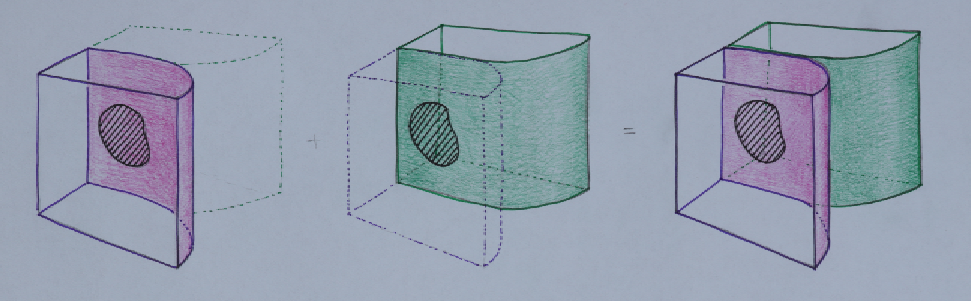
\includegraphics[width=\textwidth]{abb/extraordinaer.png}
            \caption[Eine extraordinäre Raumentität als Summe zweier ordinärer Flächenregionen]{Eine extraordinäre Raumentität als Summe zweier ordinärer Flächenregionen.\\
            Die schraffierten Teile koinzidieren, überlappen jedoch nicht.}
            \label{fig:extraordinaer}
        \end{figure}
        %
		Diese Konstruktion mag auf den erste Blick künstlich erscheinen, es lassen sich jedoch auch im Alltag Beispiele finden, die belegen, dass es sinnvoll ist, von der Existenz extraordinärer Raumentitäten auszugehen. 
		Man nehme beispielsweise ein Buch. 
		Zugeklappt erscheint es bei erster Betrachtung als Quader. 
		Wichtiger ist jedoch, was auf den Seiten steht, d.\,h.\ nicht der Quader und eigentlich auch nicht die Buchseiten, sondern die Oberfläche der Buchseiten sind das Interessante an diesem Objekt. 
		Diese Oberflächen koinzidieren für je zwei gegenüberliegende Seiten.
		Selbstverständlich macht es keinen Sinn, diese koinzidierenden Flächen zu identifizieren, da sie verschiedene Informationen enthalten. 
		Die Oberfläche eines Buches als mereologische Summe der Oberfläche seiner Seiten besitzt also jede Menge koinzidierender nichtgleicher Teile und ist somit eine extraordinäre Raumentität.
        %
		Da Raumregionen nicht koinzidieren können, sind sie immer ordinär.
		
		
		%Im Folgenden werde ich die Theorie der ordinären Raumentitäten $\BSO$ nennen. Sie enthält die selben primitiven Relationen wie $\BS$. Die hier vorgestellten Interpretationen sollen Modelle dieser Theorie sein. Insofern ergeben sich ihre Axiome aus der gewählten Interpretation.
		
    \paragraph{Zusammenhang:}
        Zusammenhängende
        \marginpar{($d$-dimensional) zusammenhängend} 
        Raumentitäten sind Raumentitäten, in denen -- anschaulich gesprochen -- je zwei Punkte (als Hyperteile) durch einen \glqq Weg\grqq\ in ihrem Inneren verbunden werden können.
        Je nach Art der \glqq schwächsten\grqq\ Verbindungsstelle unterscheiden wir $2$-, $1$- und $0$-dimensional zusammenhängende Raumentitäten (siehe Abbildung \ref{fig:zusammenhang}).
        Genauer gesagt: Eine Raumentität ist $d$-dimensional zusammenhängend, wenn jeder Schnitt, der sie in zwei Teile zerlegt, mindestens Dimension $d$ hat.%
        \footnote{
            Dieser Zusammenhangsbegriff ist nicht zu verwechseln mit dem topologischen Begriff des $d$-Zusammenhangs, der auf Homotopieklassen beruht.
        }
        Jede $d$-dimensional zusammenhängende Raumentität ist also auch ($d$-1)-dimensional zusammenhängend.
        Man beachte, dass Raumregionen auch dann $d$-dimensional zusammenhängend sein können, wenn sie lokal Stellen mit schwächerem Zusammenhang haben. Dieses Konzept wird im Anhang \ref{sec:lok-zusammenhang} als Nebenresultat formalisiert. Siehe hierzu auch das Beispiel für eine $1$-dimensional zusammenhängende Flächenregion in Abbildung \ref{fig:zusammenhang}.

        \begin{figure}[ht]
            \centering
            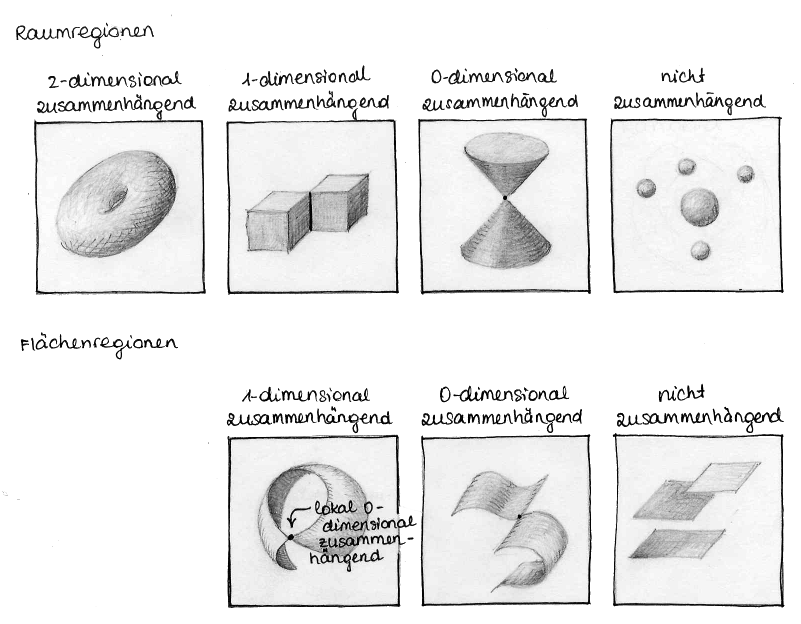
\includegraphics[width=\textwidth]{bearbeitet-22-04-25/zusammenhang_2.png}
            \caption{Verschieden zusammenhängende Raumentitäten}
            \label{fig:zusammenhang}
        \end{figure}
    
    \paragraph{Topoide, Flächen, Linien und Punkte:}
        Eine
        \marginpar{Topoid,\\Fläche,\\Linie,\\Punkt}
        $2$-dimensional zusammenhängende Raumregion heißt Topoid (topoid).
        Eine $1$-di\-men\-sional zusammenhängende ordinäre Flächenregion heißt Fläche (surface).
        Eine zusammenhängende ordinäre Linienregion heißt Linie (line).
        Eine atomare %\footnote{Eine Entität ist atomar, wenn sie keine echten Teile besitzt (d.h., wenn sie nur sich selbst als Teil besitzt).} 
        Punktregion heißt Punkt (point).
        Topoide, Flächen, Linien und Punkte sind die Raumentitäten, die unserer Intuition am nächsten kommen.
        Sie sind ordinär
        %\footnote{Man beachte, dass Raumregionen und atomare Raumentitäten immer ordinär sind.}
        und global gesehen maximal-dimensional zusammenhängend.
        Man beachte jedoch, dass sie lokal möglicherweise schwächer zusammenhängend sein können, wie in Abbildung \ref{fig:zusammenhang} das Beispiel für eine $1$-dimensional zusammenhängende Flächenregion.

% Every continuum exhibits certain basic features: it has a boundary, it does not 
% possess atomic parts, and for any division of it into two non-overlapping parts
% each of them possesses a boundary, such that these boundaries are distinct and
% coincide.
% It follows that any continuum is connected; there are no jumps or gaps in it. 
% Moreover, in our framework continua cannot be adequately modeled by sets of 
% points (e.g., of the Euclidean space $\mathbb{R}^3$).
% Space continua are classified into being 1-dimensional, called lines, 
% 2-dimensional, being connected surfaces, and 3-dimensional, called topoids.
%
% -> Kontinua müssen keinen Rand haben (beispielsweise die Oberfläche einer Kugel)
% -> aus den genannten Eigenschaften folgt nicht, dass Kontinua ordinär sein müssen
		
% besagen, sicherstellen, ausdrücken, aussagen, sagen, bedeuten, implizieren
    
\section{Axiome}\label{ssec:axiome}
%Eine vollständige Liste der $\BS$-Axiome findet sich im Anhang \ref{}. 
%Hier werden die wichtigsten Inhalte dieser Axiome ausgeführt.
$\theoryBS$ liegt als Axiomatisierung in 33 Axiomen vor, die auf den Übersichtsblättern (Übersicht 1) aufgelistet sind.
In diesem Abschnitt fasse ich ihre wichtigsten Aussagen zusammen.

Die
%\marginpar{Grundlegende Taxonomie und Existenz,\\$\Gspart$}
ersten Axiome (A1--A3) stellen sicher, dass es Raumentitäten gibt und dass diese je nach Dimension in vier paarweise disjunkte Klassen zerfallen.
A4--A7
%\marginpar{Mereologische Überlegungen}
garantieren, dass die $\Gspart$-Relation eine Äquivalenzrelation für gleichdimensionale Raumentitäten ist.


Wenn
%\marginpar{Starkes Ergänzungsprinzip}
eine Raumentität $A$ eine andere ($B$) nicht komplett einschließt%
\footnote{im Sinne der $\Gspart$-Relation},
so gibt es einen Rest -- also eine Raumentität, die Teil von $A$ ist und nicht mit $B$ überlappt (siehe Abbildung \ref{fig:supplementation}).
Diese Eigenschaft heißt starkes Ergänzungsprinzip (strong supplementation principle) und wird in A8 formalisiert.

\begin{figure}[ht]
    \centering
    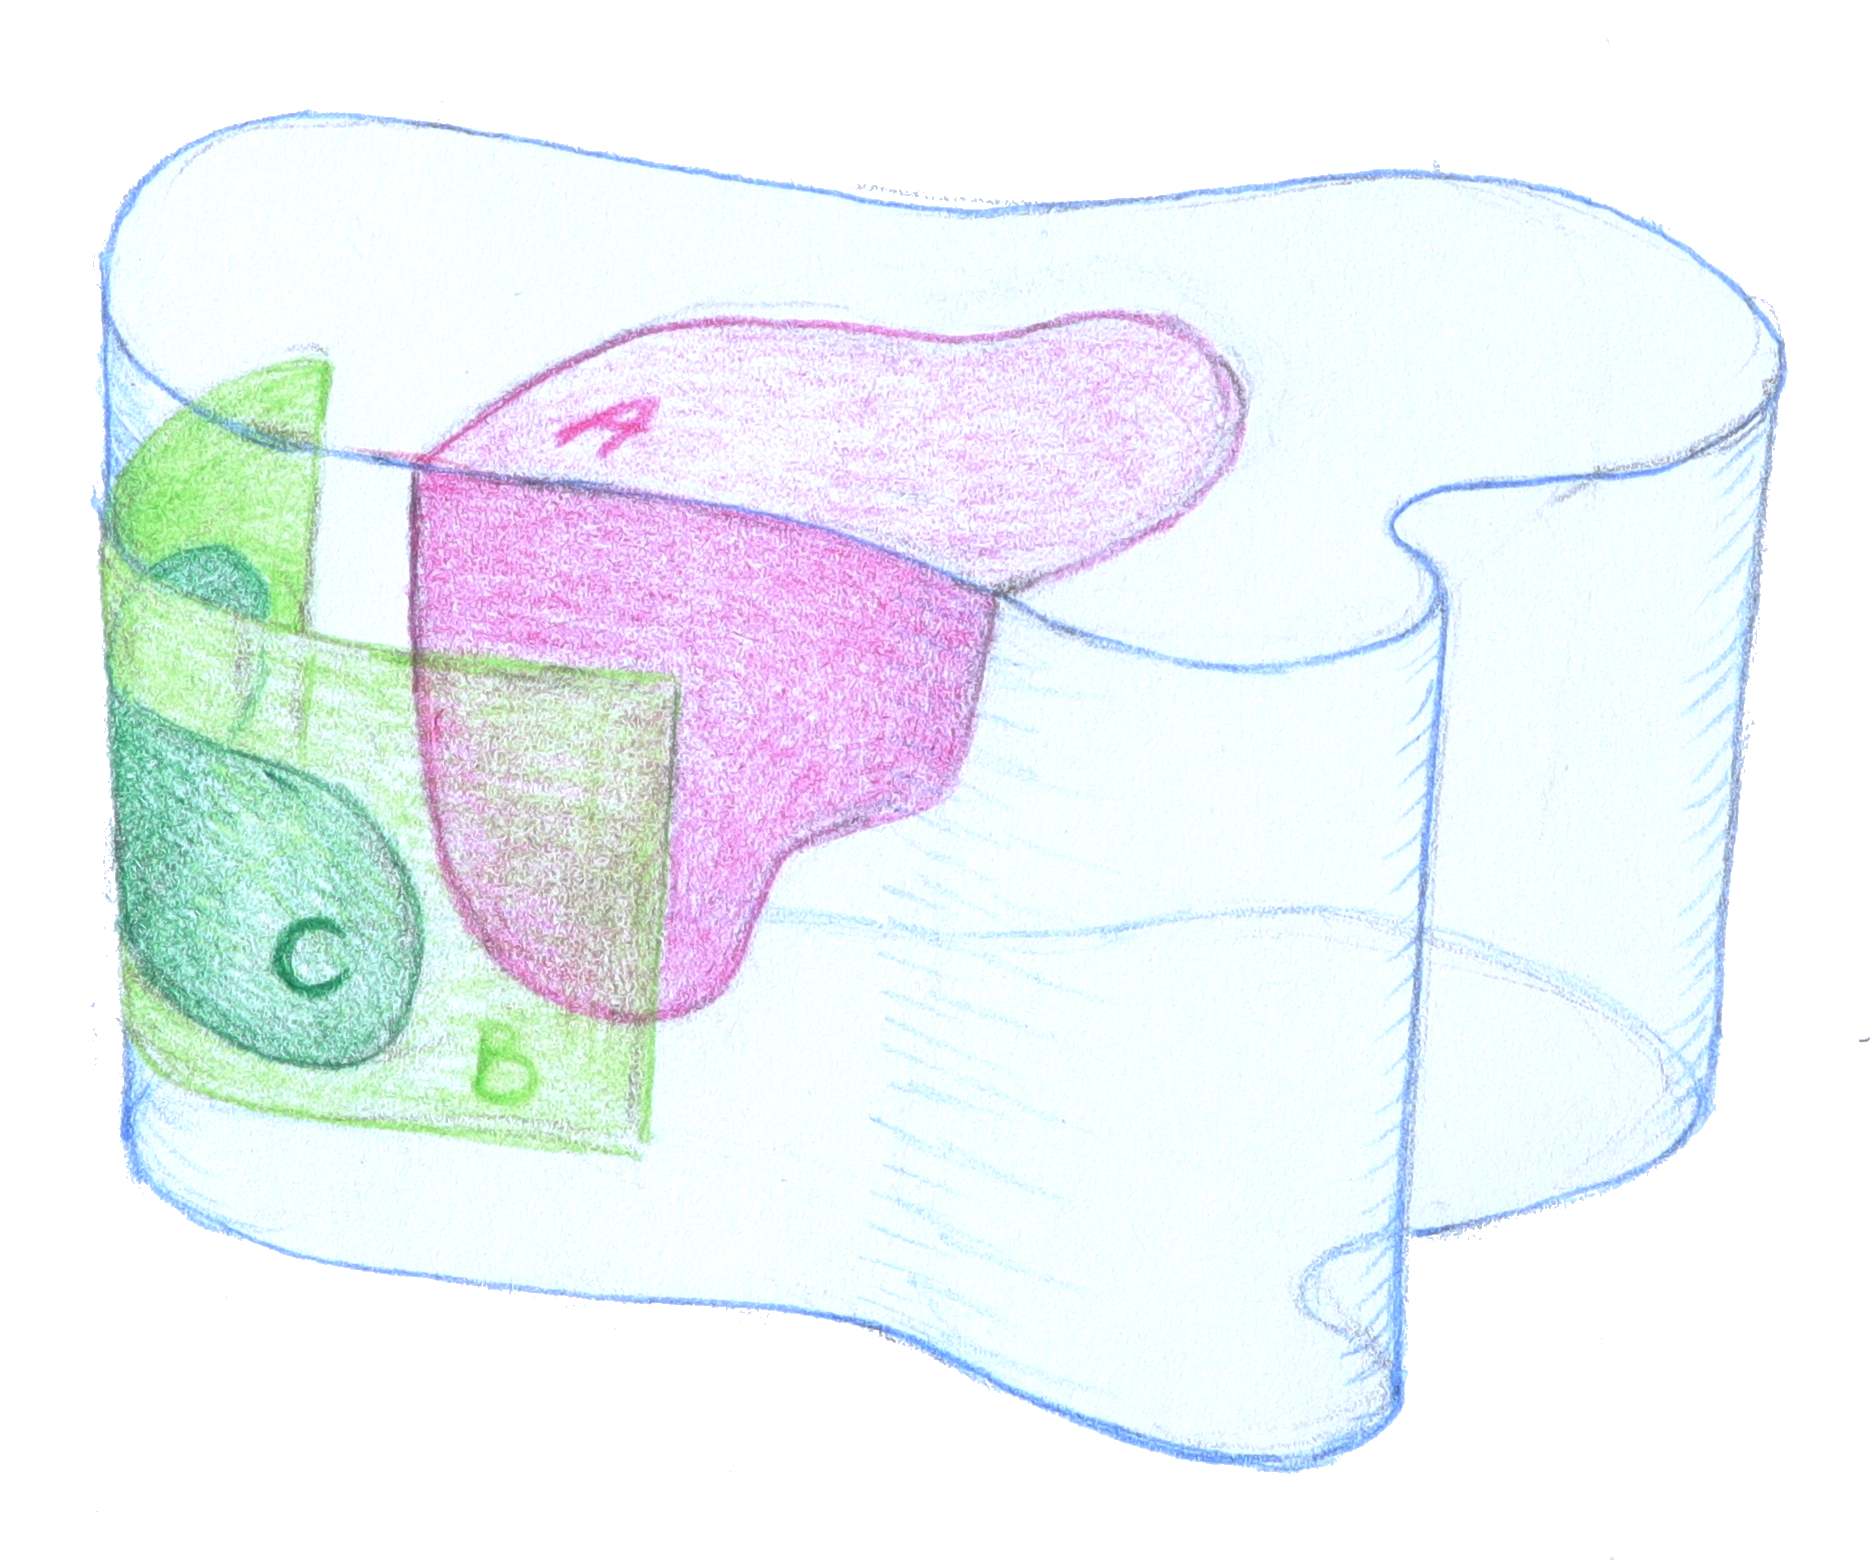
\includegraphics[height=5cm]{abb/supplementation.png}
    \caption[Zum starken Ergänzungsprinzip]{Zum starken Ergänzungsprinzip: $A$ ist nicht Teil von $B$, deshalb gibt es einen Teil $C$ von $B$, der nicht mit $A$ überlappt.}
    \label{fig:supplementation}
\end{figure}

% Das starke Ergänzungsprinzip (strong supplementation principle) (A8) bedeutet, dass wenn eine Raumentität $A$ eine andere ($B$) nicht komplett einschließt (im Sinne der $\Gspart$-Relation), muss es einen Rest geben, der für die Differenz von $A$ und $B$ verantwortlich ist -- also eine Raumentität, die in $A$ liegt und nicht mit $B$ überlappt.

% Intuitively, this says that if an object fails to include another among its parts, then there must be a remainder, something that makes up for the difference. 

A9--A10
%\marginpar{Einschränkung und Erweiterung von Raumentitäten}
sorgen dafür, dass jede Raumentität -- mit Ausnahme von Punktregionen -- einschränkbar und erweiterbar ist. D.\,h., sie besitzt einen echten inneren Teil und ist in eine echt größere einbettbar. Letzteres gilt auch für Punktregionen.
Zusammen mit A1 ergibt sich daraus insbesondere, dass jedes $\theoryBS$-Modell unendlich ist.

A11--A18
%\marginpar{Existenz von Raumentitäten} 
sind Existenzaxiome. 
Sie garantieren, dass jede Raumregion in ein Topoid einbettbar ist und geben Bedingungen für die Existenz (größter) räumlicher Grenzen, der mereologischen Summe, des Schnitts und des relativen Komplements zweier Raumentitäten an.
Hervorzuheben ist hierbei Axiom A16, das die uneingeschränkte Existenz mereologischer Summen für gleichdimensionale Raumentitäten fordert.

Dass
%\marginpar{$\Gscoinc$}
die $\Gscoinc$-Relation auf gleichdimensionalen räumlichen Grenzen eine Äquivalenzrelation ist, wird durch die Axiome A19--A22 ausgedrückt.

A23
%\marginpar{$\Gsb$}
besagt, dass ordinäre Raumentitäten ordinäre Grenzen haben.
A24 garantiert, dass Teile von Grenzen wieder Grenzen der selben Raumentitäten sind.
A25 und A26 enthalten weitere Aussagen über die $\Gsb$-Relation.
A25 hat einen wichtigen Einfluss auf die Definition der Objektäquivalenz in Kapitel~\ref{chap:bso-struktur}, die die Grundlage des vorgestellten Interpretationsansatzes bildet.
Es hat zur Folge, dass eine Raumentität $A$, die eine zweite ($B$) begrenzt, auch jede andere Raumentität begrenzt, die \glqq aus dem Inneren von $B$ auf $A$ zukommt\grqq .
Siehe hierzu Abbildung \ref{fig:A25}.
A27--A30
%\marginpar{Koinzidenz und unterscheidbare Hyperteile}
geben Eigenschaften der $\Gspart$- und $\Ghypp$-Relation an.


    \begin{figure}[ht]
        \centering
        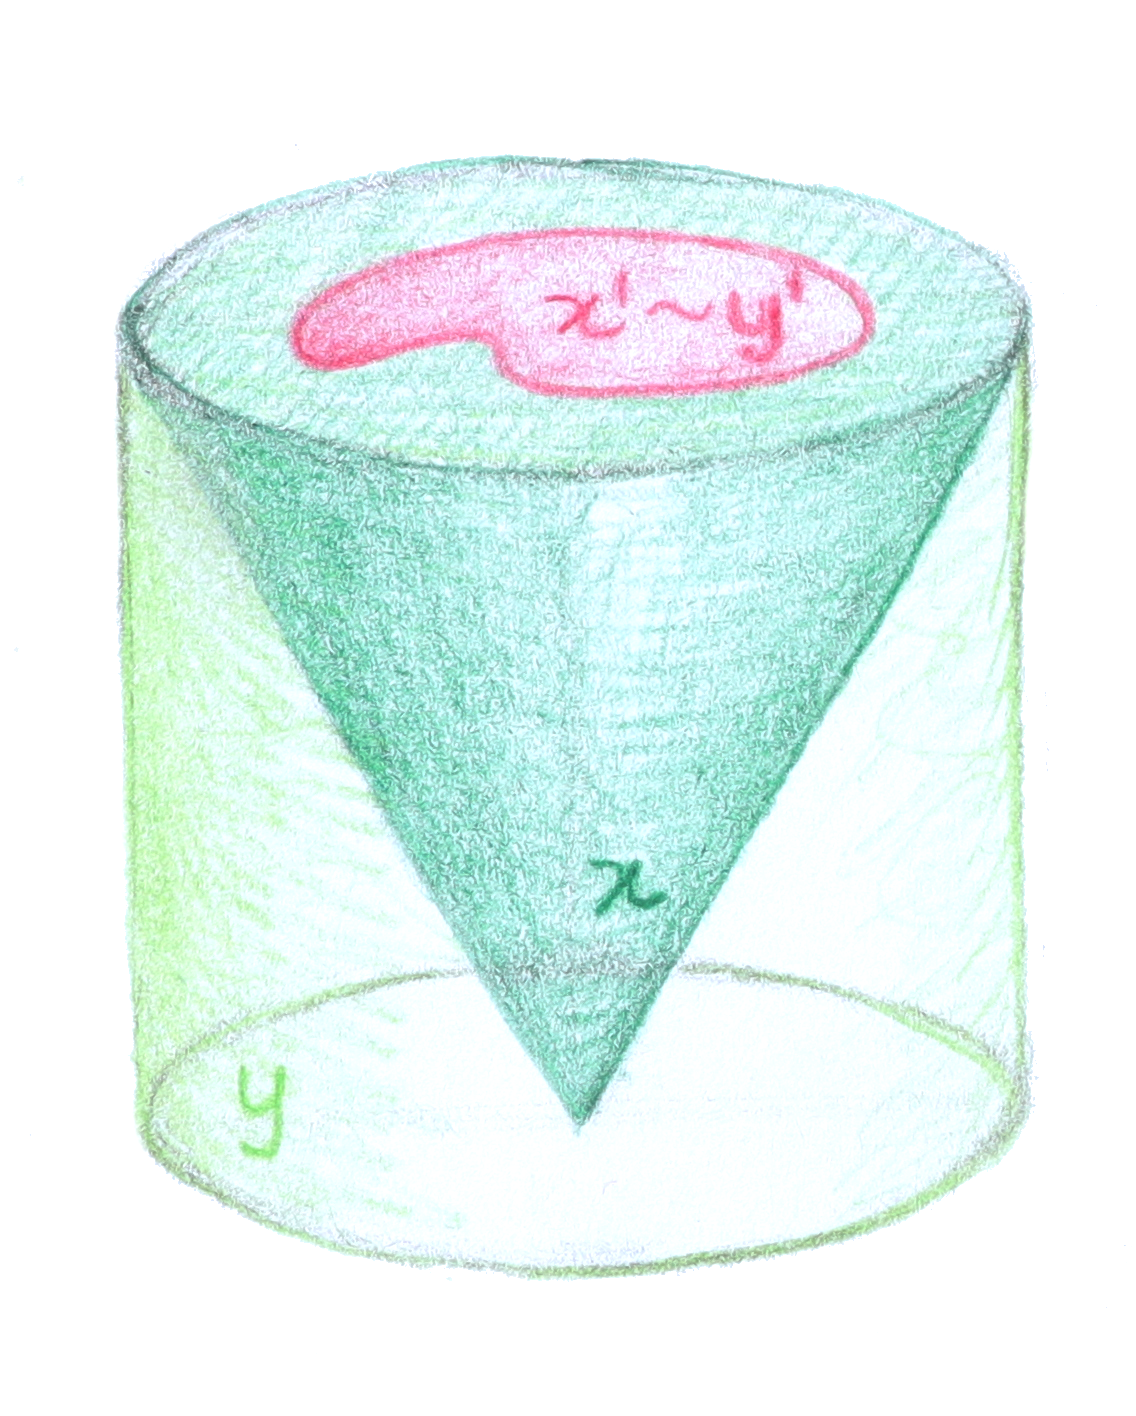
\includegraphics[height=5cm]{abb/a25.png}
        \caption[Zu Axiom 25]{Zu Axiom A25: Wenn $x$ in $y$ liegt und $x'$ (Grenze von $x$) und $y'$ (Grenze von y) koinzidieren, so begrenzt $x'$ auch $y$.}
        \label{fig:A25}
    \end{figure}
    
    In
    %\marginpar{(Un)Gleichheit von räumlichen Grenzen}
    einem 2019 von denselben Autoren veröffentlichten Konferenzpapier [\cite{baumann-r-2019--a}] werden drei weitere Axiome eingeführt, die wichtige Vorstellungen widerspiegeln, die dem hier vorgestellten Interpretationsansatz zugrunde liegen.
    
    Nach Axiom A31 besitzen Raumentitäten, die eine gemeinsame Grenze haben, einen gemeinsamen echten Teil an dieser Grenze.
    
    Der Erläuterung zu A32 in [\cite{baumann-r-2019--a}] entsprechend zielt Axiom A32
		analog auf eine Art Umkehrung von A31 ab,
		indem an unterschiedlichen Grenzen die begrenzten Entitäten disjunkte Teile 
		mit diesen Grenzen aufweisen sollen.
    %\marginpar{Diskussion zu Axiom A32}
    A32 muss jedoch formal modifiziert werden, da es in der gegebenen Form nicht der intendierten Aussage entspricht. Ein problematischer Fall ist in Abbildung \ref{fig:a32} dargestellt.
    
    \begin{figure}[ht]
        \centering
        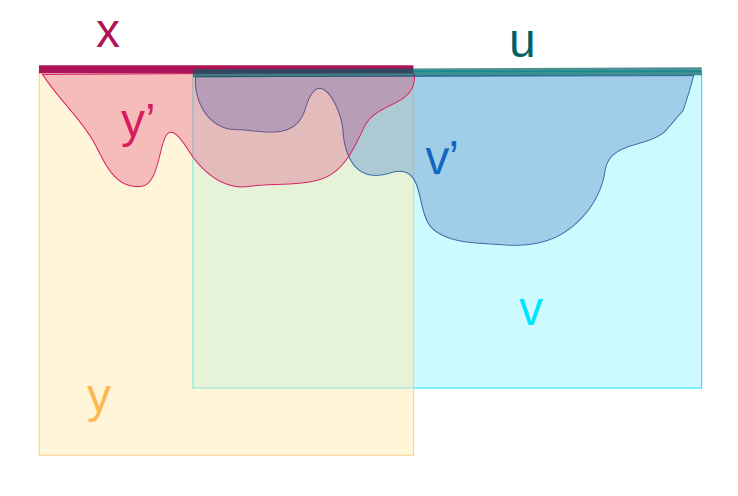
\includegraphics[height=3.5cm]{gfx/a32.png}
        \caption[Zu Axiom 32]{Zu Axiom A32: Zwei Grenzen, für die je zwei Raumentitäten, die von ihnen begrenzt werden, überlappen}
        \label{fig:a32}
    \end{figure}
    
    In der ursprünglichen Version lautet das Axiom:
%     \begin{align*}
%         &\Gsb(x,y) \land \Gsb(u,v) \land x\neq u \to\\ 
%         &\exists y'v'\:(\: \Gspart(y',y) \land \Gsb(x,y') \land \Gspart(v',v) \land \Gsb(u,v') \land \neg \Gsov(y',v'))
%     \end{align*}
    \begin{align*}
        \Gsb(x,y) \land \Gsb(u,v) \land x\neq u &\to\: 
        \exists y'v'\:(\: \Gspart(y',y) \land \Gsb(x,y') 
        \land \mbox{} \\
        &\Gspart(v',v) 
        \land \Gsb(u,v') \land \neg \Gsov(y',v'))
    \end{align*}

    
    Angenommen, es gibt Raumentitäten $x$, $y$, $u$ und $v$ mit $\Gsb(x,y)$, $\Gsb(u,v)$, $x \neq u$ und $\Gsov(x,u)$ und A32 gilt.
    Seien $y'$ und $v'$ Raumentitäten mit $\Gspart(y',y)$, $\Gsb(x,y')$, $\Gspart(v',v)$, $\Gsb(u,v')$ und $\neg \Gsov(y',v')$.
    Nach der Definition von $\Gsov$ gibt es eine Raumentität $z$ mit $\Gspart(z,x)$ und $\Gspart(z,u)$.
    Damit gelten nach Axiom A24
    %\marginpar{FL, 22.04.: TODO\\neu A24 war A23 - bitte nochmal checken} 
    $\Gsb(z,y')$ und $\Gsb(z,v')$ und somit existiert nach Axiom A31 eine Raumentität $w$ mit $\Gsppart(w,y')$ und $\Gsppart(w,v')$.
    Also überlappen $y'$ und $v'$. $\lightning$
    
    Deshalb schlage ich vor, $x \neq u$ zu $\neg \Gsov(x,u)$ zu verschärfen.
% 
% $$\Gsb(x,y) \wedge \Gsb(x,z) \to
%              \exists u (\Gsb(x,u) \land \Gsppart(u,y) \land \Gsppart(u,z))$$
% % 				 \label{ax:cbspp}}
% %        {entities with a common boundary share a proper part at that boundary}	
% % 						
% % 						
% % \itemTP{ \mbox{}$\\
% % \hspace*{1em}
% %
% $$\Gsb(x,y) \land \Gsb(u,v) \land x\neq u \to \exists y'v'\:(\: \Gspart(y',y) \land \Gsb(x,y') \land \Gspart(v',v) \land \Gsb(u,v') \land \neg \Gsov(y',v')) $$
% 			  \label{ax:dbipno}}
%        {entities with distinct boundaries have parts at those boundaries
% 			  that do not overlap}
% 				
% \itemTP{$\GLDE(x) \Land \GOrd(x) \Limp \GSB(x)$\\ \mbox{}

    A33
    %\marginpar{Ordinäre Raumentitäten und Grenzen}
    schließlich besagt, dass alle ordinären niederdimensionalen Raumentitäten räumliche Grenzen sind.
    Damit sind die Forderungen
    \begin{enumerate}
     \item \glqq Alle Raumentitäten sind ordinär.\grqq\ und
     \item \glqq Alle niederdimensionalen Raumentitäten sind räumliche Grenzen.\grqq
    \end{enumerate}
    äquivalent.


    
\section{Die Theorie der ordinären Raumentitäten}\label{sec:bso}
Um die Konstruktion eines Modells zu erleichtern, führe ich in dieser Arbeit die vereinfachte Raumtheorie $\theoryBSO$ ein, die nur räumliche Grenzen als niederdimensionale Raumentitäten zulässt.
% \cFLs Die Ontologie $\BS^O$ ist eine Vereinfachung von $\BS$, die nur räumliche Grenzen als niederdimensionale Raumentitäten zulässt.\cFLimp{Einstieg anpassen: Ab hier neue Definition von $\BS^O$ und weswegen, dann die eigentliche Darstellung/Einführung von $\BS^O$}
Unter dieser Voraussetzung besteht das Diskursuniversum nur aus Raumregionen und räumlichen Grenzen.
Aus Axiom A23, das besagt, dass räumliche Grenzen von ordinären Raumentitäten wieder ordinär sind, folgt damit, dass alle Raumentitäten ordinär sind.
% Wenn alle niederdimensionalen Raumentitäten räumliche Grenzen sind,
% das Diskursuniversum also nur aus Raumregionen und räumlichen Grenzen besteht,
% dann sind alle Raumentitäten ordinär.
% Dies ist im Wesentlichen eine Folgerung aus Axiom A23, das besagt, dass räumliche Grenzen von ordinären Raumentitäten wieder ordinär sind.
Deshalb ist $\theoryBSO$ die Theorie der ordinären Raumentitäten.

Da durch mereologische Summenbildung extraordinäre Raumentitäten entstehen können, muss die Gültigkeit von Axiom A16 eingeschränkt werden, das die Existenz der mereologischen Summe für gleichdimensionale Raumentitäten fordert.

\paragraph{Axiomatisierung}\ \\
$\theoryBSO$ entsteht aus $\theoryBS$ durch die Hinzunahme eines weiteren Axioms
$$\text{A0.} \quad \GLDE(x) \to \GSB(x)$$
und Modifikation von A16 zu
\begin{align*}
 \text{A16'.} \quad \Geqdim(x,y) \wedge \mbox{} &\neg \exists x'y'\ (\Gspart(x',x) \wedge \Gspart(y',y) \wedge \mbox{} \\
 &\Gscoinc(x',y') \wedge \neg \Gsov(x',y')) \to \exists z\ \Gsum(x,y,z)
\end{align*}

%\todo[inline]{\small FL n03.05. mini\\
%$\neg sov(x,y)$ in A16' könnte vor die mit $\neg \exists x' y'$ beginnende Teilformel gezogen werden, da dieses Literal nur $x$ und $y$ betrifft.
%Fiel mir nur neu auf; bei Änderung erneute Angabe am Ende von 2.4 beachten.\\
%-> BH: Ich denke, du hast da eher einen Fehler entdeckt und es müsste $\neg sov(x',y')$ heißen}
A16' besagt, dass die Existenz der mereologischen Summe zweier gleichdimensionaler Raumentitäten dann garantiert ist, wenn diese keine koinzidierenden, nichtüberlappenden Teile besitzen -- wenn also durch die Summenbildung keine extraordinäre Raumentität entsteht.
Ob diese Einschränkung ausreicht und ob gegebenenfalls noch weitere Axiome eingeschränkt werden müssen, ist noch zu untersuchen (vgl.\ dazu die Diskussion in Abschnitt \ref{sec:offene-fragen}).

Abbildung \ref{fig:summe-linien} zeigt ein Beispiel für die mereologische Summe zweier Linienregionen, die nicht extraordinär ist und somit auch nach Axiom A16' existiert.
Dargestellt sind zwei Linienregionen $x$ und $y$, die die Flächenregionen $x'$ und $y'$ begrenzen.
Ihre mereologische Summe ist wiederum Grenze einer Raumentität $z'$, die sich jedoch nicht durch einfache Mengenoperatoren aus $x'$ und $y'$ konstruieren lässt.
Allerdings gilt, dass $x$ und $y$ auch $z'$ begrenzen.

\begin{figure}[ht]
    \centering
    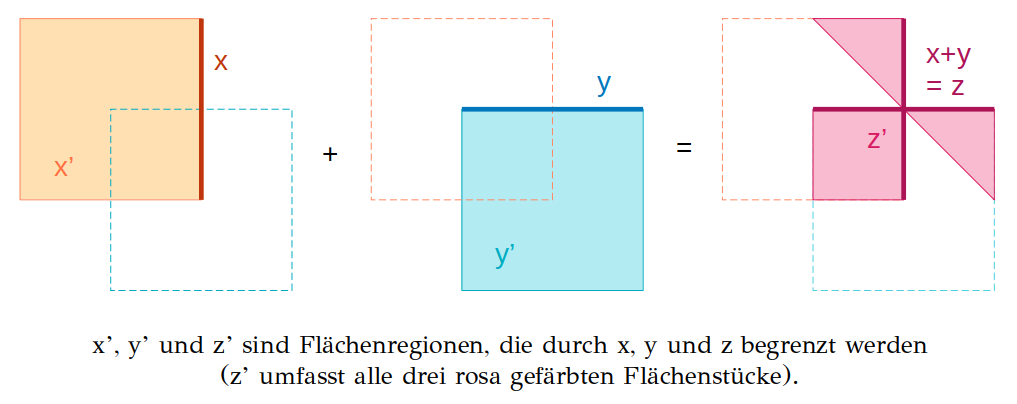
\includegraphics[width=0.9\textwidth]{gfx/summe-linien.png}
    \caption{Beispiel für die mereologische Summe zweier Linienregionen, die \textit{nicht} extraordinär ist}
    \label{fig:summe-linien}
\end{figure}

%\todo[inline]{\small FL n03.05. mini\\
%Im Text in Abb.\ \ref{fig:summe-linien} ``rosa gefärbte'' $\to$ ``rosa gefärbten''\\
%-> BH: done}
Als Folgerung aus dem neuen Axiom A0 und den alten Axiomen A2, A3 und A23 sowie den Definitionen D22 und D23 ergibt sich, dass in $\theoryBSO$ alle Raumentitäten ordinär sind. $\theoryBSO$ enthält also als zusätzliches Theorem
$$ \GOrd(x). $$
Dadurch ist das Konzept ordinärer Raumentitäten in der Theorie $\theoryBSO$ trivialisiert. Insgesamt bietet sich aus derartigen Gründen eine Modifikation der Theorie an.

\paragraph{Modifizierte Formalisierung}\ \\
Durch die Einschränkung von $\theoryBS$ auf $\theoryBSO$ werden einige Definitionen vereinfacht bzw. überflüssig, da sie triviale Konzepte definieren oder da definierte Konzepte zusammenfallen.
Dies führt auch dazu, dass Axiome umgeschrieben werden müssen, die besagte Konzepte enthalten. 
Andere werden tautologisch und können deshalb entfallen.
Eine vollständige Liste aller Symbole und Axiome findet sich auf den beiliegenden Übersichtsblättern (Übersicht 2).

%\paragraph{Definitionen}\ \\
D7 und D8 sind redundant, weil $\GLDE$ mit $\GSB$ und $\GdDE$ mit $\GdDB$ zusammenfallen.\\
Durch Ersetzung von $\GdDE$ durch $\GdDB$ wird aus D9
\begin{align*}
 \text{D9'.} \quad \Geqdim(x) := 
      &(\GSReg(x) \wedge \GSReg(y)) \vee (\GtwoDB(x) \wedge \GtwoDB(y)) \vee \mbox{} \\ 
			&(\GoneDB(x) \wedge \GoneDB(y)) \vee (\GzeroDB(x) \wedge \GzeroDB(y))
\end{align*}
%
D22 und D23 können gestrichen werden, da $\GExOrd$ und $\GOrd$  in $\theoryBSO$ triviale Konzepte sind.\\
%
Die Definitionen für Topoid, Fläche, Linie und Punkt vereinfachen sich zu  
%
\begin{align*}
 &\text{D30'.} \quad \GTop(x) := \GSReg(x) \wedge \GtwoDC(x)\\
 &\text{D31'.} \quad \GtwoD(x) := \GtwoDB(x) \wedge \GoneDC(x)\\
 &\text{D32'.} \quad \GoneD(x) := \GoneDB(x) \wedge \GzeroDC(x) \\
 &\text{D33'.} \quad \GzeroD(x) := \GzeroDB(x) \wedge \neg \exists y\ \Gsppart(y,x)
\end{align*}
%
%\paragraph{Axiome}\ \\
%Durch die Ersetzung von $\GLDE$ durch $\GSB$, $\GExOrd$ durch $\bot$ und $\GOrd$ durch $\top$ verändern sich einige Axiome bzw. sie werden überflüssig.
%
Das in diesem Abschnitt eben erst eingeführte zusätzliche Axiom A0 kann wegfallen, wenn $\GLDE$ durch $\GSB$ ersetzt wird.\\
%
A2 und A3 werden zu
\begin{align*}
 &\text{A2'.} \quad \GSB(x) \leftrightarrow \neg \GSReg(x)\\
 &\text{A3'.} \quad \neg \exists x\ ((\GtwoDB(x) \wedge \GoneDB(x)) \vee (\GtwoDB(x) \wedge \GzeroDB(x))\\
 &\phantom{\text{A3'.} \quad \neg \exists x\ ((} \vee (\GoneDB(x) \wedge \GzeroDB(x)))
\end{align*}
%
A13 und A14 müssen modifiziert werden und A15 vereinfacht sich zu
\begin{align*}
 &\text{A13'.} \quad \GtwoDB(x) \to \exists yz\ (\Gsppart(y,x) \wedge \Gsb(y,z))\\
 &\text{A14'.} \quad \GoneDB(x) \to \exists yz\ (\Gsppart(y,x) \wedge \Gsb(y,z))\\
 &\text{A15'.} \quad \exists y\ \Gsb(y,x) \to \exists z\ \Ggrsb(z,x)
\end{align*}
%
A16 wird nicht vereinfacht, sondern die Bedingung für die Existenz der mereologischen Summe wird verschärft zu dem schon erwähnten Axiom
\begin{align*}
 \text{A16'.} \quad \Geqdim(x,y) \wedge &\neg \exists x'y'\ (\Gspart(x',x) \wedge \Gspart(y',y) \wedge \\
 &\Gscoinc(x',y') \wedge \neg \Gsov(x',y')) \to \exists z\ \Gsum(x,y,z)
\end{align*}
%
A23 ($\Gsb(x,y) \wedge \GOrd(x) \to \GOrd(y)$) schließlich lässt sich ersatzlos streichen.
